%% document class
\documentclass[10pt]{beamer}
%%theme
\usetheme[hideothersubsections,width=2cm]{Berkeley}
%% page settings
\usepackage{xcolor}
\usenavigationsymbolstemplate{}
\usefonttheme{serif}

%% packages
\usepackage{courier}
\usepackage{geometry}
\usepackage{graphicx}
\usepackage[scaled=0.9]{helvet}
\usepackage{multimedia}
\usepackage{mathptmx}
\usepackage{tikz}

%%color settings
%%%%% Color Schema

\definecolor{blue_dark}{RGB}{38,50,56}
\definecolor{blue}{RGB}{33,150,243}
\definecolor{blue_light}{RGB}{79,195,247}
\definecolor{grey_dark}{RGB}{38,50,56}
\definecolor{grey}{RGB}{33,150,243}
\definecolor{grey_light}{RGB}{33,150,243}

%% theme settings
\setbeamercolor*{palette primary}{fg=grey_dark,bg=blue_light} % upper part
\setbeamercolor*{palette secondary}{fg=grey_dark,bg=blue_light} % left part (background)
\setbeamercolor*{sidebar left}{fg=blue_light,bg=grey_dark} % left part with links
\setbeamercolor*{palette sidebar primary}{fg=blue_light}
\setbeamercolor*{palette sidebar secondary}{fg=blue_light}
\setbeamerfont{section in sidebar}{size=\scriptsize}

%% new commands
%\input{settings/macros}
\addtobeamertemplate{frametitle}{\vskip+0.6ex}{}
\makeatletter
\beamer@headheight=2\baselineskip
\makeatother

\begin{document}

\author[Group 9]{Suvojit Manna\\Pronab Mukherjee\\Barun Gupta\\Somnath Rakshit\\}
\title[Machine Learning]{Introduction to Machine Learning using \LaTeX}
%\logo{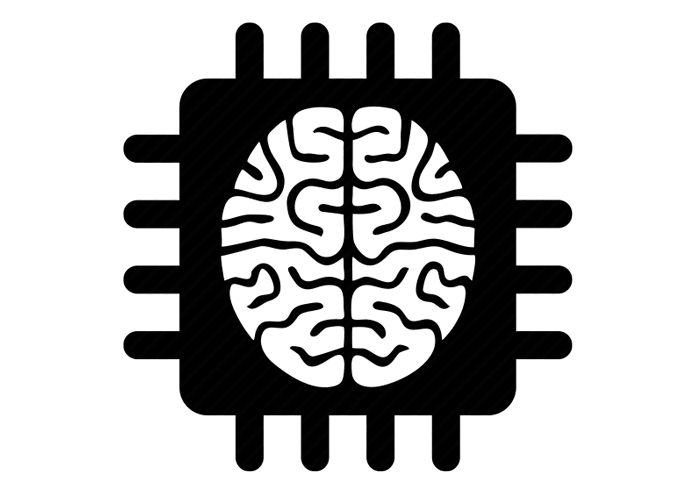
\includegraphics[width=4mm]{images/icon}}
\institute[JGEC]{Jalpaiguri Govt Engineering College}
%\date{City, date}


%% Title Page
\begingroup
\setbeamercolor{background canvas}{bg=blue_dark}
\begin{frame}[plain,t]
	\hspace*{-22 mm}
	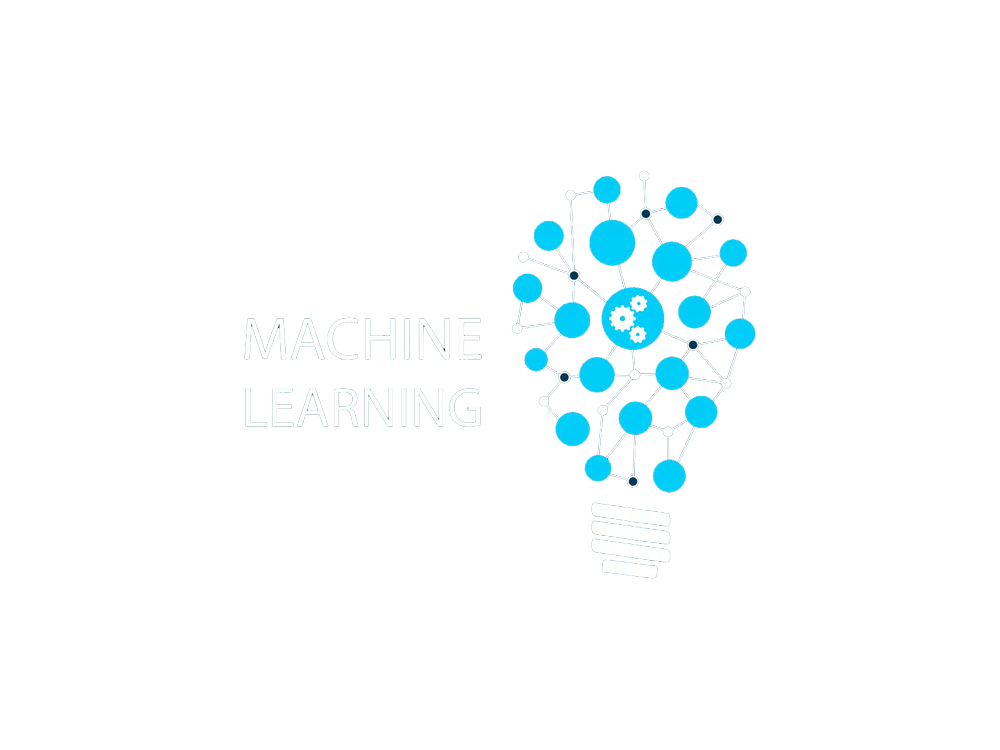
\includegraphics[width=\paperwidth,height=\paperheight]{images/ml_bg}
\end{frame}
\endgroup

%% A Team Page
\begingroup
	\usebackgroundtemplate{%
		\tikz\node[opacity=0.3] {
\includegraphics[height=\paperheight,width=\paperwidth]{images/bg-vec}}
		;}
	\begin{frame}[c]{The A Team}
		\begin{center}
			\Huge{Presented By:\\}
			\large{~\\Suvojit Manna\\Pronab Mukherjee\\Barun Gupta\\Somnath Rakshit\\}
		\end{center}
	\end{frame}
	%% contents
	\begin{frame}{Contents in Brief}
		%\tableofcontents
		\tableofcontents[hideallsubsections]
	\end{frame}
\endgroup
	%% Big Font Page: Lets get started
\begingroup
	\setbeamercolor{background canvas}{bg=blue_dark}
	\setbeamercolor{normal text}{fg=blue_light}
	\begin{frame}[plain,c]
		\hspace*{10 mm}
		\vspace*{-18 mm}
		\textcolor{blue_light}{\Huge{Let's Get Started}}
	\end{frame}
\endgroup


\begingroup
	\usebackgroundtemplate{%
		\tikz\node[opacity=0.3] {
\includegraphics[height=\paperheight,width=\paperwidth]{images/bg-vec}}
		;}
	
	\section{Introduction}
		\begin{frame}{Machine Learning | What ?}
			\begin{center}
				\large{Field of study that gives computers the ability to learn without being explicitly programmed.}\\
				\bigskip
				\small{Instead of writing code, you feed data to the generic algorithm and it builds its own logic based on the data.}
				\begin{figure}
				\centering
				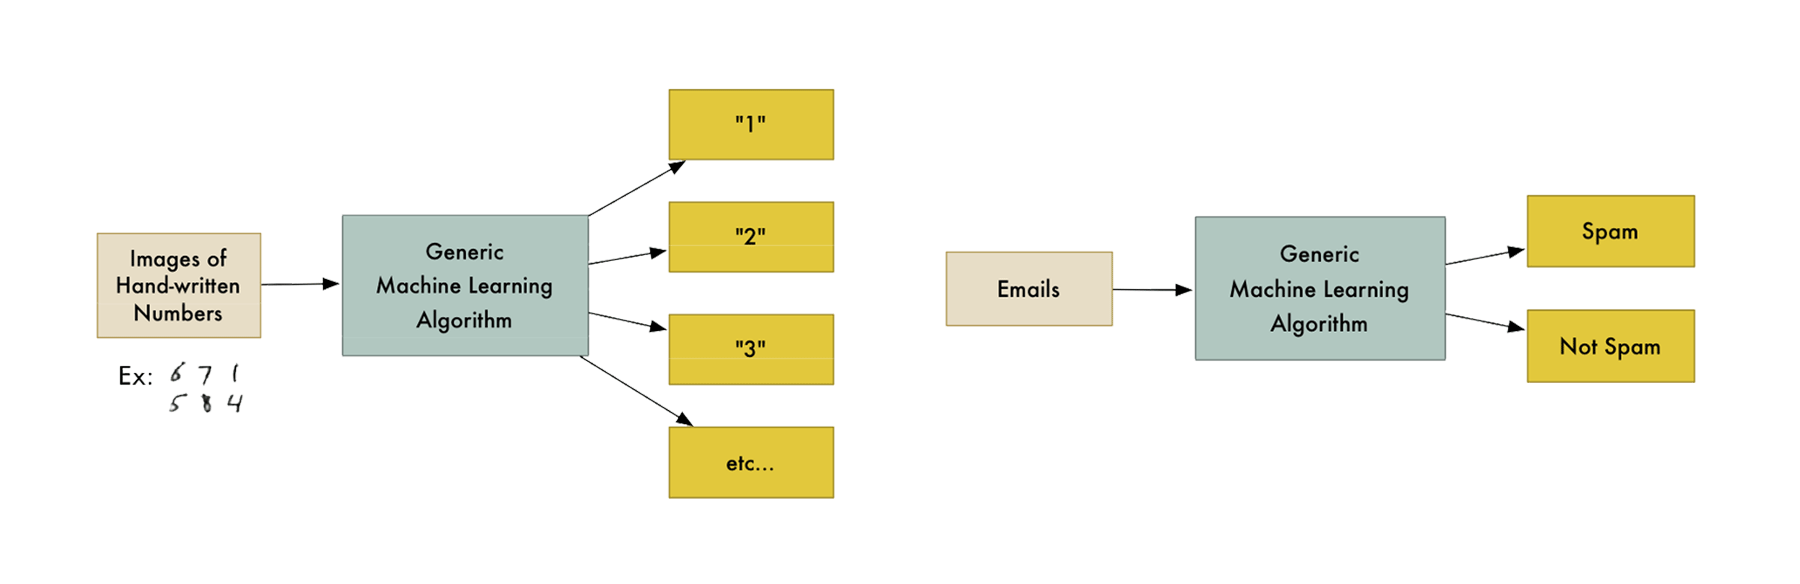
\includegraphics[width=\linewidth,height=30mm]{images/classif-ex}
				\caption[This machine learning algorithm is a black box that can be re-used for lots of different classification problems.]{Classification Algorithms}
				\end{figure}
			\end{center}
		\end{frame}
		\subsection{Case Studies}
			\begin{frame}{Case Studies | Supervised Learning}
				\begin{center}
					\begin{tabular}{|c|c|c|c|}							\hline 
						\bfseries{Bedroom} & \bfseries{Sq.Ft} & \bfseries{Neighbourhood} & \bfseries{Price}\\ 	\hline
						3       & 2000  & Uptown        & \$350,000 \\ 	\hline 
						2       & 800   & Downtown      & \$200,000 \\ 	\hline 
						2       & 850   & City Centre   & \$150,000 \\ 	\hline 
						1       & 550   & Suburbs       & \$75,000 \\	\hline 
						4       & 2000  & Suburbs       & \$200,000 \\	\hline 
					\end{tabular}\\
					\bigskip
					\begin{tabular}{|c|c|c|c|}							\hline 
						\bfseries{Bedroom} & \bfseries{Sq.Ft} & \bfseries{Neighbourhood} & \bfseries{Price}\\ 	\hline
						3   	& 2000  & Uptown        & ???\\			\hline 
					\end{tabular} \\
					\bigskip
					\begin{block}{Definiton}
						Supervised learning is the machine learning task of inferring a function from labeled training data.
					\end{block}
				\end{center} 
			\end{frame}
			\begin{frame}{Case Studies | Supervised Learning}
				\begin{center}
					\begin{tabular}{|l l|}\hline 
						\multicolumn{2}{|c|}{\textbf{Math's Exam - Answer Keys}}\\
						1) 2  4  5 = 3 & 5) 6  2  2 = 10 \\ 
						2) 5  2  8 = 2 & 6) 3  1  1 = 2  \\ 
						3) 2  2  1 = 3 & 7) 5  3  4 = 11 \\ 
						4) 2  2  4 = 6 & 8) 1  8  1 = 7  \\ \hline
					\end{tabular}\\
					\bigskip
					\begin{itemize}
						\item The training data consist of a set of training examples.
						\item Training Data :
							\begin{itemize}
								\item Input Object : Set of Features
								\item Desired Output : Supervisory Signal
							\end{itemize}
						\item A supervised learning algorithm produces an inferred function.
						\item An analogus task in human and animal phsycology : Concept Learning.
					\end{itemize}
				\end{center}
			\end{frame}
			\begin{frame}{Case Studies | Unsupervised Learning}
				\begin{center}
					\begin{figure}
					\centering
					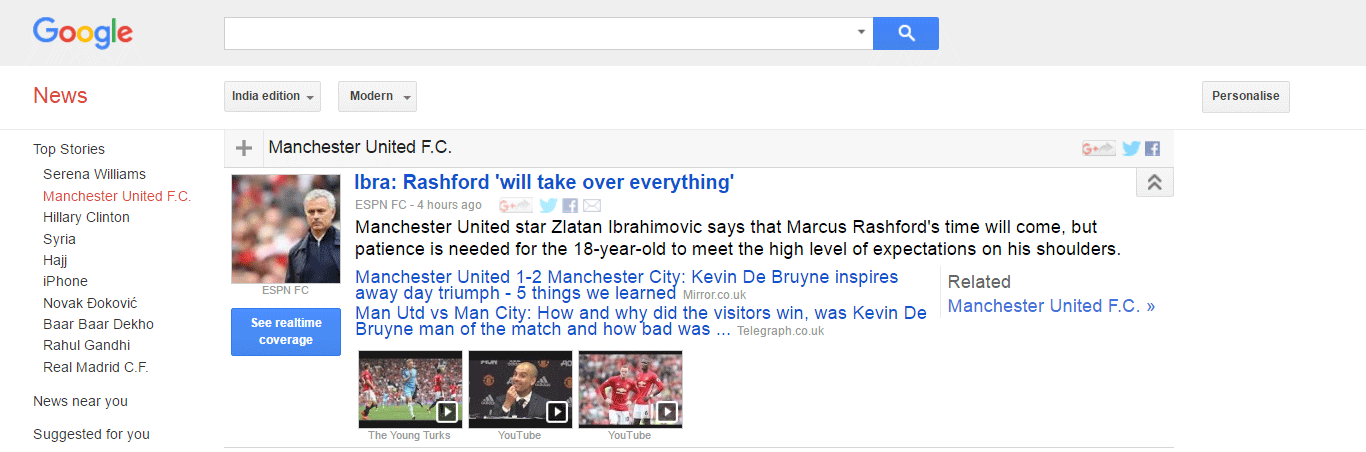
\includegraphics[width=\linewidth]{images/unsupl-ex}
					\caption{Google News grouping similar stories together.}
					\end{figure}
					\begin{block}{Definiton}
						Unsupervised learning is the machine learning task of inferring a function to describe hidden structure from unlabeled data.
					\end{block}
				\end{center}
			\end{frame}
			\begin{frame}{Cocktail Party Problem | Unsupervised Learning}
				\begin{columns}
					\begin{column}{0.5\textwidth}
						Sound from :
						\begin{itemize}
							\item \sound[label=show1, inlinesound]{{\it Microphone 1}}{sounds/cpp-mix1.wav}
							\item \sound[label=show1, inlinesound]{{\it Microphone 2}}{sounds/cpp-mix2.wav}
						\end{itemize}
						\bigskip
						Output from Learning Algorithm :
						\begin{itemize}
							\item \sound[label=show1, inlinesound]{{\it Output 1}}{sounds/cpp-output1.wav}
							\item \sound[label=show1, inlinesound]{{\it Output 2}}{sounds/cpp-output2.wav}
						\end{itemize}
					\end{column}
					\begin{column}{0.5\textwidth}
						\begin{figure}
							\centering
							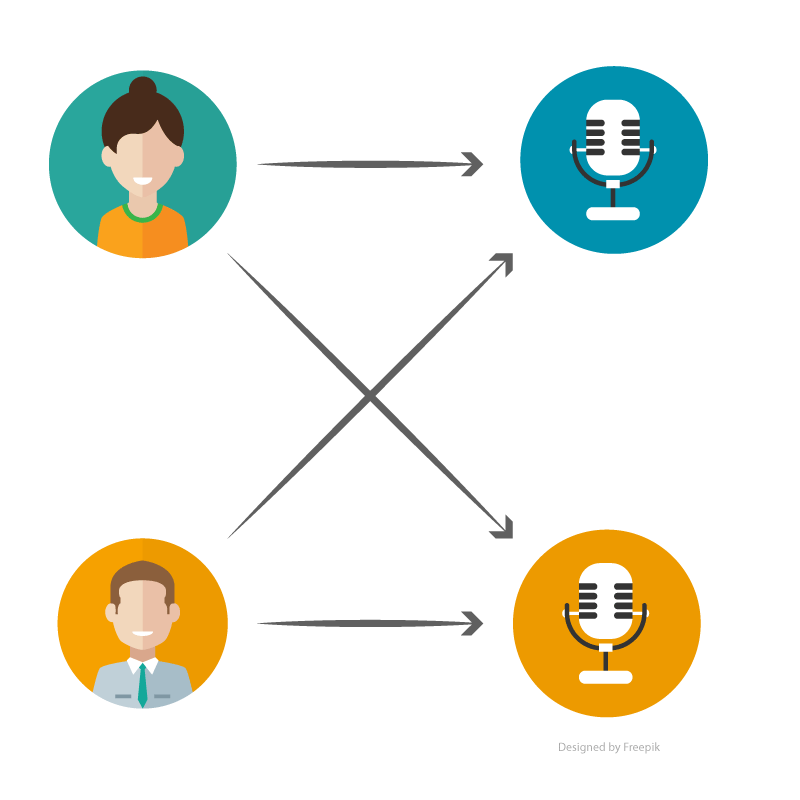
\includegraphics[width=1.0\linewidth]{images/cpp-repr}
							\caption{Overlapped Recordings}
						\end{figure}
					\end{column}
				\end{columns}
			\end{frame}
			\begin{frame}{Case Studies | Unsupervised Learning}
				\begin{center}
					\begin{figure}
						\centering
						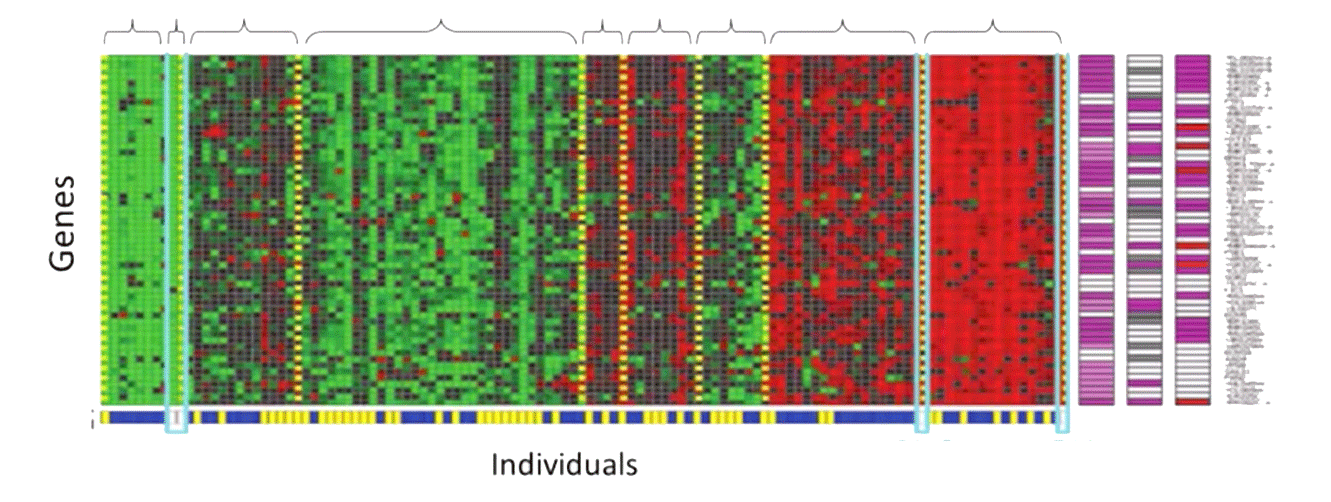
\includegraphics[width=\linewidth]{images/gene-classification}
						\caption[Gene Clustering]{Gene Clustering}
					\end{figure}
					\begin{itemize}
						\item Training Data given to the learner is unlabeled.
						\item No error or reward signal to evaluate a potential solution.
						\item Closely related to density estimation in statistics.
					\end{itemize}
				\end{center}
			\end{frame}
		\subsection{Formal Defintion}
			\begin{frame}{Machine Learning | Formal Definiton}
				\begin{center}
					\small{The field of machine learning is concerned with the question of how to construct computer programs that automatically improve with experience.}\\
					\bigskip
					\large{A computer program is said to learn from experience E with respect to some class of tasks T and performance measure P, if its performance at tasks in T, as measured by P, improves with experience E.}\\
					\bigskip
					\small{Evolved from :}
					\begin{itemize}
						\item {\small Pattern Recognition}
						\item {\small Computational Learning Theory}
						\item {\small Artificial Intelligence}
					\end{itemize}
				\end{center}
			\end{frame}
		\subsection{Applications}
			\begin{frame}{Industry Trends}
				\begin{columns}
					\begin{column}{0.5\textwidth}
						\begin{center}
						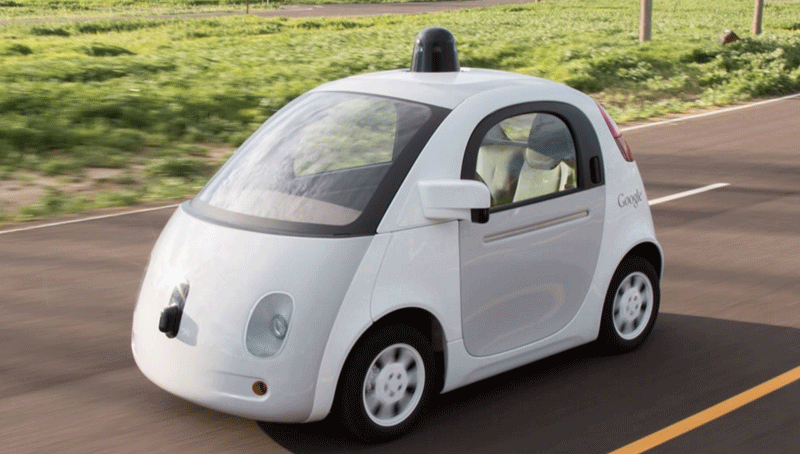
\includegraphics[width=0.9\linewidth]{images/app-2}
						\end{center}
					\end{column}
					\begin{column}{0.5\textwidth}
						\begin{center}
							Google Chauffer :
						Self Driving Car by Google
						\end{center}
					\end{column}
				\end{columns}
				\begin{columns}
					\begin{column}{0.5\textwidth}
						\begin{center}
							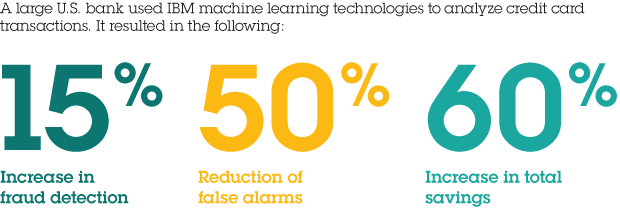
\includegraphics[width=0.9\linewidth]{images/app-3}
						\end{center}
					\end{column}
					\begin{column}{0.5\textwidth}
						\begin{center}
							IBM Research : Credit Card Fraud Detection
						\end{center}
					\end{column}
				\end{columns}
				\begin{columns}
					\begin{column}{0.5\textwidth}
						\begin{center}
							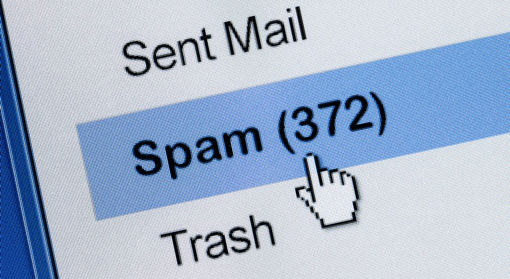
\includegraphics[width=0.9\linewidth]{images/app-5}
						\end{center}
					\end{column}
					\begin{column}{0.5\textwidth}
						\begin{center}
							Mail Services : Spam Filtering
						\end{center}
					\end{column}
				\end{columns}
			\end{frame}
			\begin{frame}{Industry Trends}
				\begin{figure}
					\centering
					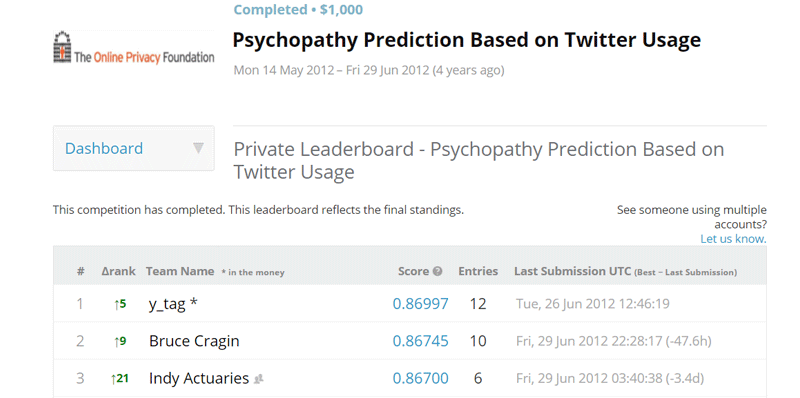
\includegraphics[width=0.9\linewidth]{images/app-1}
					\caption{Kaggle Challenge : Psychopathy Prediction}
				\end{figure}
				\begin{center}
					The  aim of the competition is to determine to what degree it's possible to predict people with a sufficiently high degree of Psychopathy based on Twitter usage and Linguistic Inquiry.
				\end{center}
			\end{frame}
			\begin{frame}{Entertainment | Machine Learning}
				%TODO : Insert MarI/O video
			\end{frame}
			\begin{frame}{Applications | Machine Learning}
				\begin{columns}
					\begin{column}{0.5\textwidth}
						\begin{itemize}
							\item Adaptive websites
							\item Classifying DNA sequences
							\item Computer vision
							\item Internet fraud detection
							\item Natural language processing
						\end{itemize}
					\end{column}
					\begin{column}{0.5\textwidth}
						\begin{itemize}
							\item Online advertising
							\item Recommender systems
							\item Search engines
							\item Sentiment analysis
							\item Speech and handwriting recognition
						\end{itemize}
					\end{column}
				\end{columns}
				%TODO : Insert Animation	
			\end{frame}
		\subsection{Benefits}
			\begin{frame}{Machine Learning | Why ?}
				\begin{columns}
					\begin{column}{0.5\textwidth}
						\begin{itemize}
							\item Can work with huge amount of data.
							\item Can make intelligent decisions by taking into account multiple features.
							\item Can find patterns in large amount of data which is almost impossible for human beings. 
							\item These algorithms are self-modifying in nature, they get better over time as the usage increases.
						\end{itemize}
					\end{column}
					\begin{column}{0.5\textwidth}
						\begin{center}
							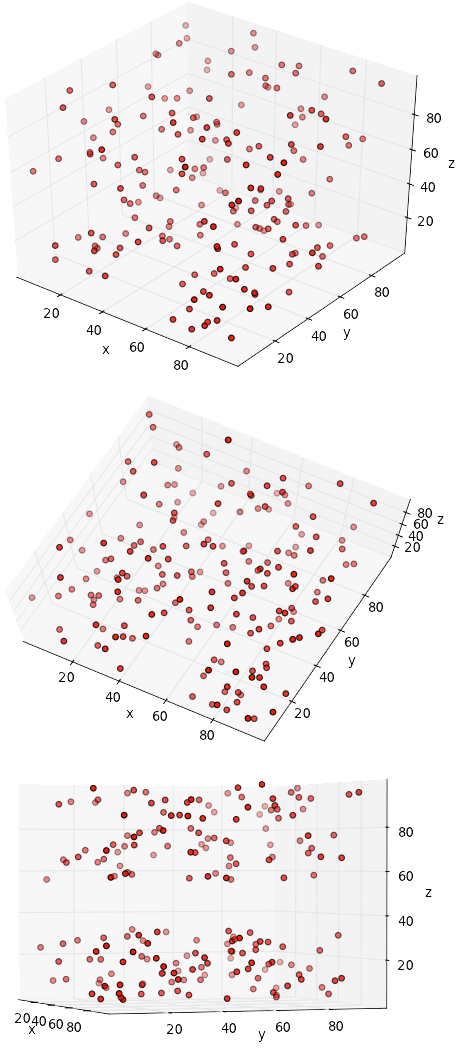
\includegraphics[height=0.9\textheight]{images/pca-merge}
						\end{center}
					\end{column}
				\end{columns}
			\end{frame}	
	\section{Regression}
		\begin{frame}{Introduction | Regression}
		\end{frame}
		\subsection{Usages}
			\begin{frame}{Usages | Regression}
			\end{frame}
		\subsection{Benefits}
			\begin{frame}{Benefits | Regression}
			\end{frame}
		\subsection{Example Cases}
			\begin{frame}{Example Cases | Regression}
			\end{frame}
	
	\section{Classifications}
		\begin{frame}{Introduction | Classifications}
		\end{frame}
		\subsection{Usages}
			\begin{frame}{Usages | Classifications}
			\end{frame}
		\subsection{Example Cases}
			\begin{frame}{Example Cases | Classifications}
			\end{frame}
	
	
	\section{Deep Learning}
		\begin{frame}{Introduction | Deep Learning}
		\end{frame}
		\subsection{Neural Networks}
			\begin{frame}{Neural Networks | Deep Learning}
			\end{frame}
		\subsection{Meaning}
			\begin{frame}{Meaning | Deep Learning}
			\end{frame}
		\subsection{Usages}
			\begin{frame}{Usages | Deep Learning}
			\end{frame}
		\subsection{Advantages}
			\begin{frame}{Advantages | Deep Learning}
			\end{frame}
	
	
	
	\section{Conclusion}
		\begin{frame}{The pain is almost over}
		\end{frame}
		\begin{frame}{Bibliography}
			\twocolumn
			\begin{itemize}
				\item \scriptsize{Phil Simon (March 18, 2013). Too Big to Ignore: The Business Case for Big Data. Wiley. p. 89. ISBN 978-1-118
					-63817-0.}
				\item \scriptsize{Mitchell, T. (1997). Machine Learning, McGraw Hill. ISBN 0-07-042807-7}
				\item \scriptsize{ Mehryar Mohri, Afshin Rostamizadeh, Ameet Talwalkar (2012) Foundations of Machine Learning, The MIT Press ISBN 9780262018258.}
				\item \scriptsize{Jordan, Michael I.; Bishop, Christopher M. (2004). "Neural Networks". In Allen B. Tucker. Computer Science Handbook, Second Edition (Section VII: Intelligent Systems). Boca Raton, FL: Chapman \& Hall/CRC Press LLC. ISBN 1-58488-360-X.}
				\item \scriptsize{https: //www.kaggle.com/c/twitter-psychopathy-prediction}
				\item \scriptsize{Mastering the game of Go with deep neural networks and tree search (2016), D. Silver et al.}
			\end{itemize}
			\onecolumn
		\end{frame}
\endgroup

\begingroup
	\setbeamercolor{background canvas}{bg=blue_dark}
	\setbeamercolor{normal text}{fg=blue_light}
	\begin{frame}[plain,c]
		\hspace*{6 mm}
		\vspace*{-18 mm}
		\textcolor{blue_light}{\Large{Now that was very interesting!}}
	\end{frame}
	\begin{frame}[plain,c]
		\hspace*{27 mm}
		\vspace*{-20 mm}
		\textcolor{blue_light}{\Large{The End}}
	\end{frame}
\endgroup

\end{document}


